\documentclass[main.tex]{subfiles}
\begin{document}
\chapter{Introduction}
	\section{The ATmega328p}

	The ATmega328p is a microcontroller designed by $\mathrm{Atmel}^{\copyright}$.
	It is an 8-bit microcontroller with two 8-bit counters, an analog-to-digital
	converter, 4 GPIO ports (23 GPIO pins total) and 32 $\mathrm{kBytes}$ of
	programmable memory. This project uses the following features:

		\begin{enumerate}
			\item 8-bit timer
			\item Analog-to-digital Converter
			\item 2 GPIO Ports 
		\end{enumerate}

	\section{Analog To Digital Conversion}\label{sec:ADC}
	The ATmega328p has a ten bit successive approximation analog to digital
	converter (or ADC). Successive approximation is an analog to digital
	conversion method in which the input signal is constantly compared to the
	output of a guessed analog value (\figref{adcSA} shows this process). After
	all n bits of the converter are set the ADC interrupt service routine (or ADC
	ISR) is called (see \secref{tempConvIfcSec} for details on the ADC ISR). 

	\begin{figure}[H]
		\begin{center}
			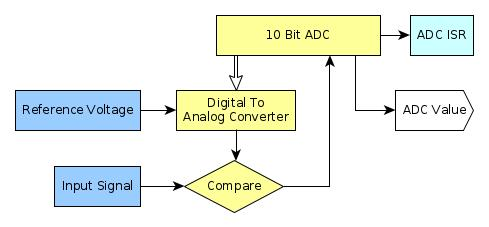
\includegraphics[width=\linewidth]{adc}
		\end{center}
		\caption{ADC Successive Approximation}
		\label{fig:adcSA}
	\end{figure}

	The result from an ADC conversion is a 10 bit number (known as an ADC value)
	that represents the input voltage. The maximum and minimum ADC values
	represent $V_{ref}$ and $\mathrm{GND}$ respectively.
		
	\section{Temperature Measurement}
	A thermistor is a resistor in which its resistance is a function of
	temperature. When the thermistor is placed in a parallel circuit as shown in
	\figref{parallelThermistor} the value of $V_{out}$ become a function (see
	\eqref{Vout})of $R_{1}$ (the thermistor). Because $R_{1}$ varies with
	temperature this makes $V_{out}$ a function of temperature as well and can
	then be used to calculate a ``sensed'' temperature.
	
	\begin{equation}
		V_{out}(R_{1}) = \frac{V_{cc}R_{2}}{R_{1}+R_{2}}
		\label{eq:Vout}
	\end{equation}
	
	\begin{figure}[H]
		\begin{center}
			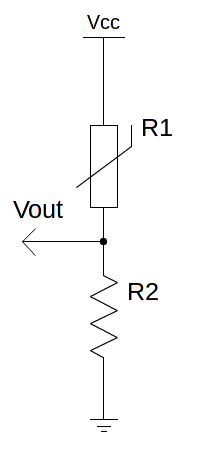
\includegraphics[width=0.25\linewidth]{thermParallel}
		\end{center}
		\caption{Thermistor ($R_{1}$) in Parallel}
		\label{fig:parallelThermistor}
	\end{figure}
	
	There does not exist a universal function that maps voltage to temperature.
	Instead a table is created and once a voltage is measured linear interpolation
	is used to calculate a temperature. \tabref{sampleData} shows a sample table.
	The data in the temperature and resistance columns are unique to the
	thermistor being used and can obtained from the thermistor's datasheet. The
	data in the voltage column was created using~\eqref{Vout} (where $V_{cc} = 5$
	and $R_{1} = 1\mathrm{k}\Omega$). The ADC column data are the resulting ADC values
	for their corresponding $V_{out}$.

	\begin{table}[H]
		\begin{center}
			\csvautobooktabular[
				after table=\caption{Sample Temperature Conversion Data}\label{tab:sampleData},
				table head=\toprule\
				Temp($^{\circ}\mathrm{C}$) & $R_{1}$($\mathrm{k}\Omega$) & $V_{out}$ & ADC\\
				\midrule\csvlinetotablerow\\
					%$R_{1}$\left($\mathrm{k}\Omega$\right)
					 %$V_{out}$
					%ADC
			]{../sampleTemp.csv}
		\end{center}
	\end{table}
	
	\section{Linear Interpolation}\label{sec:linearInterpolation}
	Linear interpolation is a method of estimating the values in between entries
	of a data table (in this case \tabref{sampleData}).  To find interpolated
	values based on a desired value (in this case an ADC value) the two
	``nearest'' data points are chosen and a linear function is formed between the
	two using point-slope form:

	\[
		f(x) = \frac{(y_{2}-y_{1})}{(x_{2}-x_{1})}(x-x_{1})+y_{1}\\
	\]

	(where $\left(x_{1},y_{1} \right)$ and $\left(x_{2},y_{2}\right)$ are two
	nearest data points). 

	%The idea is two points are chosen from the table (one
	%greater than, one less than the desired value) and a linear equation is formed
	%from those two points. Then the desired function value is found by computing
	%the formed function with a desired given input value into this function.
	
	%include graph of data
	\begin{figure}[H]
		\begin{center}
			\subfile{figures/adcTempGraph.tex}
		\end{center}
		\caption{Linear Interpolation of~\tabref{sampleData}}
		\label{fig:adcTempGraph}
	\end{figure}
	
	\figref{adcTempGraph} shows the linear interpolation of~\tabref{sampleData}.
	ADC values are used for $x_{n}$ instead of $V_{out}$ because this is what the
	ATmega328p translates $V_{out}$ into (therefore converting ADC values into a
	voltage before performing a linear interpolation is inefficient). The lines
	between each data point represent the functions to be used for linear
	interpolation\footnotemark. Here is an example of computing the temperature
	for the ADC value $400$.

	\begin{enumerate}
		\item find the nearest points values to $400$ in the table: ($(343,20)$ and
			$(445,30)$)  
		\item Create the linear interpolation function:
			\[
				f(x) \equiv \frac{(30-20)}{(445-343)}(x-343)+20
			\]
		\item Compute $f\left(400 \right)$: $f(400) \approx 25.59^{\circ}\mathrm{C}$
	\end{enumerate}

	\footnotetext{Note: there are no interpolation lines past the end
		points of the table ($(241,10)$ and $(938,90)$). Interpolation beyond these
		points can be made by continuing their previous lines, however this could
		result in under/over approximation which can be dangerous in some
		applications.}

	%To perform a linear interpolation for the ADC value $400$ one
	%would and create the linear function between the two. Substituting $400$ for $x$
	%gives the corresponding temperature value ($25.59^{\circ}\mathrm{C}$).
	
	%\begin{eqnarray*}
		%& \therefore & 
	%\end{eqnarray*}
	
	%A generic equation would be:
	

	
	
	%This report is divided into two sections; the first half is for program logic
	%and the second is for hardware. The software section will cover configuration of
	%the ATmega328p's timer for updating the seven-segment display and digit
	%multiplexing, the ADC for converting the thermistors voltage signal into digital
	%data and extracting the thermistor temperature from the data. The hardware
	%extion will cover setting up the Dragon programmer, powering the Atmega and the
	%ADC, seven-segment pin layout and setup, and connecting the thermistor.
	
\end{document}
